\section{指数函数}

本节要点:
\begin{itemize}
    \item 掌握指数函数的概念及意义;
    \item 熟悉指数函数的图形。
\end{itemize}

~

指数函数
\[
y=a^x \qquad a>0\text{且}a\ne 1 \quad x\in \mathbb{R}
\]
本身非常简单,没有难度,只需要注意$a$的取值范围。$a=1$时,$y$变成常数函数$y=1$没有讨论的意义;$a<0$时,$y$为复数,较为复杂,高中阶段不讨论。

若将$x$取自然数$n\in \mathbb{N} $,则不难发现,指数函数变成了一个等比数列的通项公式。所以指数函数的意义就是将等比数列的通项公式进行“稠密化”。于是,也不难理解:
\begin{itemize}
    \item 指数函数是单调函数,具体看$a$;
    \item 当$a>1$时,单调递增,且$a$越大增速越快,曲线越陡;
    \item 当$a<1$时,单调递减,且$a$越小减速越快,曲线同样越陡。
\end{itemize}

\begin{figure}[h]
\centering
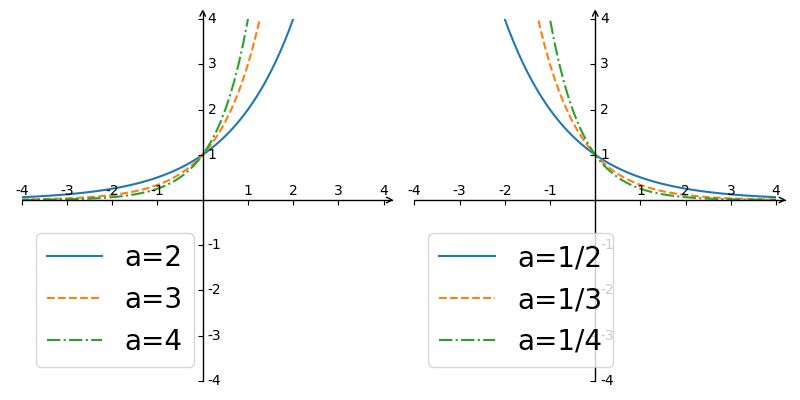
\includegraphics[height=5cm]{4.2-1.png}
\end{figure}

~

\begin{example}[拓广探索9,难度:$\star $]
已知函数
\[
y=a\left( \frac{1}{2} \right) ^{\left| x \right|}+b
\]
图象过原点,且无限接近直线$y=2$但又不与该直线相交。
\begin{enumerate}
    \item 求该函数的解析式,并画出图象;
    \item 判断该函数的奇偶性和单调性。
\end{enumerate}
\end{example}

解:

原函数可化为:
\[
y=\left( \frac{1}{2} \right) ^{\log _{1/2}a}\left( \frac{1}{2} \right) ^{\left| x \right|}+b=\left( \frac{1}{2} \right) ^{\left| x \right|+\log _{1/2}a}+b
\]
对比标准的指数有渐近线$y=0$,这里的渐近线为$y=2$,抬高了2,必然是$b$引起的,所以$b=2$。图象过原点,于是有$0=a+b$,则$a=-2$,最终:
\[
y=-2\left( \frac{1}{2} \right) ^{\left| x \right|}+2
\]
\begin{figure}[h]
\centering
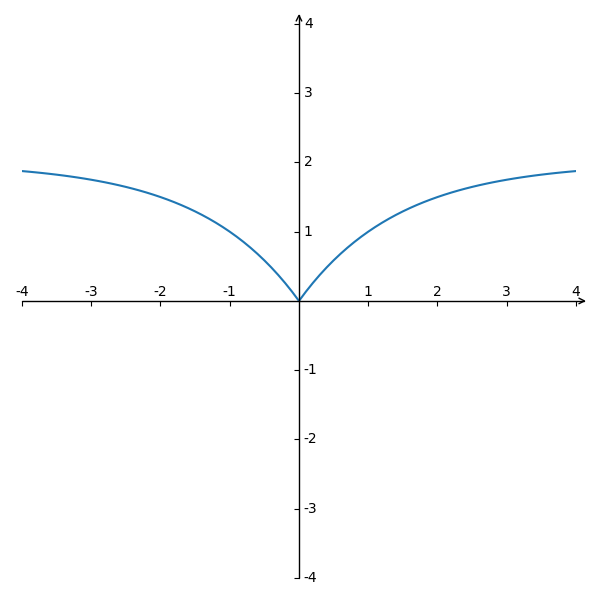
\includegraphics[height=6cm]{4.2-2.png}
\end{figure}

考察$x>0$部分函数图形从标准指数函数演化到题目所示函数的过程,函数化简如下:
\[
y=-2\left( \frac{1}{2} \right) ^x+2=-\left( \frac{1}{2} \right) ^{-1}\left( \frac{1}{2} \right) ^x+2=-\left( \frac{1}{2} \right) ^{x-1}+2
\]
图形分析:
\begin{itemize}
    \item 标准的指数函数$y=\left( 1/2 \right) ^x$;
    \item 右移得到$y=\left( 1/2 \right) ^{x-1}$;
    \item 沿{\it x}轴翻转得到$y=-\left( 1/2 \right) ^{x-1}$;
    \item 上抬2得到$y=-\left( 1/2 \right) ^{x-1}+2$。
\end{itemize}

~

~

~

~

~

~

~

\begin{figure}[ht]
\centering
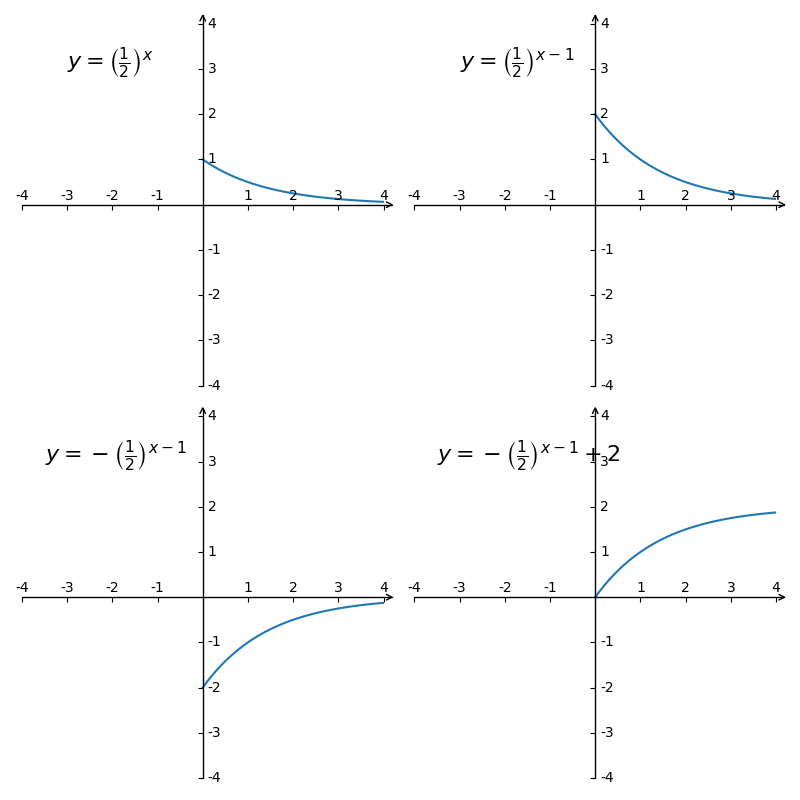
\includegraphics[height=10cm]{4.2-3.png}
\end{figure}

\begin{tcolorbox}
本题其实是对指数函数一次最完整的考察。理解一个函数如何从最基本的形态通过拉伸和平移变得复杂。
\end{tcolorbox}




